\documentclass[journal]{IEEEtran}

% ==== Packages (ASCII only; no TikZ) ====
\usepackage[T1]{fontenc}
\usepackage{lmodern}
\usepackage[utf8]{inputenc} % keep UTF-8, but write ASCII in text
\usepackage{graphicx}
\usepackage{amsmath,amssymb}
\usepackage{booktabs}
\usepackage{siunitx}
\usepackage{hyperref}
\usepackage{cite}

\graphicspath{{./}}

\title{A Comparative Review of DRAM and FeRAM: Boundary and Perspectives}

\author{Shinichi~Samizo%
\thanks{S. Samizo is with Project Design Hub (Samizo-AITL), Japan. E-mail: samizo-aitl@example.org.}
}

\markboth{Draft for IEEE-style submission}{Samizo: DRAM vs FeRAM Comparative Review}

\begin{document}
\maketitle

\begin{abstract}
This short review contrasts DRAM and FeRAM from device scaling to system use. We summarize speed, retention, endurance, energy per bit, and cell footprint, and outline how hybrid hierarchies can combine the strengths of both.
\end{abstract}

\begin{IEEEkeywords}
DRAM, FeRAM, FeFET, HfO2, retention, endurance, scaling, memory hierarchy.
\end{IEEEkeywords}

\section{Introduction}
Memory hierarchies are critical to modern computing systems. 
DRAM remains the dominant volatile memory owing to its high speed, density, and scalability~\cite{choi2022, kim2021_dram}. 
However, DRAM scaling faces fundamental challenges as the capacitor dimensions approach physical limits, particularly in sub-1z nodes~\cite{lee2020_dram, iedm2023_dram}. 
In parallel, ferroelectric HfO$_2$-based memories (FeRAM/FeFET) have emerged as promising non-volatile candidates, combining CMOS compatibility with fast switching~\cite{boscke2011, mueller2012}. 
This review targets researchers and practitioners by consolidating recent results from IEDM, VLSI, and IEEE journals, while exploring hybrid perspectives that may reshape the volatile–non-volatile boundary.


\section{DRAM Technology and Scaling}
DRAM technology has continually advanced through cell capacitor scaling, high-k dielectrics, and process innovations. 
Recent works highlight the difficulty of maintaining capacitance while suppressing leakage currents in deep sub-20 nm technologies \cite{choi2022}.
Furthermore, the industry is exploring 3D DRAM architectures to extend scaling, analogous to NAND flash, by stacking capacitor arrays \cite{kim2021_dram}.
Such approaches aim to overcome cell aspect ratio limits, though integration complexity and refresh overhead remain unresolved.

% --- sections/dram.tex の図をこの安全版に差し替え ---
\begin{figure}[!t]
\centering
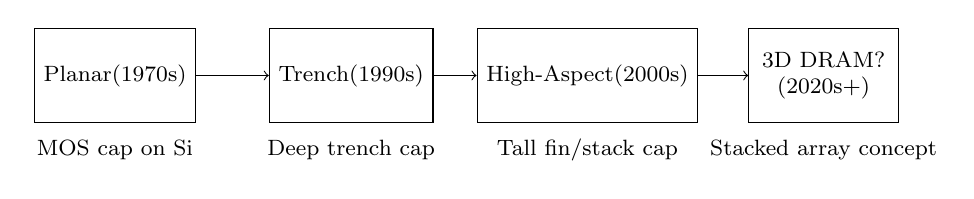
\begin{tikzpicture}[font=\footnotesize]
% ノード(座標で配置)
\node[draw, minimum width=1.9cm, minimum height=1.2cm]            (planar) at (0,0)   {Planar\\(1970s)};
\node[draw, minimum width=1.9cm, minimum height=1.2cm]            (trench) at (3,0)   {Trench\\(1990s)};
\node[draw, minimum width=1.9cm, minimum height=1.2cm]            (hac)    at (6,0)   {High-Aspect\\(2000s)};
\node[draw, minimum width=1.9cm, minimum height=1.2cm, align=center] (ddram) at (9,0)   {3D DRAM?\\(2020s+)};

% 矢印
\draw[->] (planar) -- (trench);
\draw[->] (trench) -- (hac);
\draw[->] (hac) -- (ddram);

% 注記
\node at (0,-0.95)  {MOS cap on Si};
\node at (3,-0.95)  {Deep trench cap};
\node at (6,-0.95)  {Tall fin/stack cap};
\node at (9,-0.95)  {Stacked array concept};
\end{tikzpicture}
\caption{Evolution of DRAM cell structures and concepts.}
\label{fig:dram_evolution}
\end{figure}


\section{FeRAM Technology and Advances}
The discovery of ferroelectricity in HfO$_2$ thin films~\cite{boscke2011, mueller2012} revitalized FeRAM research. 
However, retention and endurance degradation remain critical challenges~\cite{schenk2015}. 
Recent device engineering has shown improved endurance and data retention in scaled FeFETs~\cite{li2022}.


\section{Comparative Analysis}
\label{sec:comparison}
Table~\ref{tab:comparison} summarizes representative metrics for DRAM and FeRAM, including speed, retention, endurance, energy per bit, and cell footprint. 

DRAM provides ultra-high endurance ($\geq 10^{16}$ cycles) and low energy per bit, but suffers from limited retention ($\sim$64 ms) and significant refresh overhead. In contrast, FeRAM offers non-volatility with retention exceeding $10^{5}$ s and endurance in the range of $10^{12}$--$10^{13}$ cycles, though its write energy is higher (hundreds of fJ/bit) \cite{noheda2023,martin2020}. 

Fig.~\ref{fig:svr} shows the speed--retention trade-off, while Fig.~\ref{fig:evs} highlights the relationship between write energy and speed. These comparative plots illustrate that DRAM is optimal for working memory, whereas FeRAM is better suited for low-power non-volatile applications.


\section{Hybrid Perspectives}

\noindent
Hybrid hierarchies may leverage DRAM as the high-speed working set while deploying FeRAM as a near-memory non-volatile tier or NVDIMM-like layer. System-level implications include refresh-energy reduction, fast checkpointing, and resilience. Competition and complementarity with MRAM, ReRAM, PCM, and FeFET variants are also discussed in the context of endurance and energy constraints.


\section{Conclusion}
Comparative analysis suggests that DRAM will continue as the workhorse volatile memory, maintaining unmatched endurance and density. Meanwhile, FeRAM provides a compelling pathway toward embedded non-volatile solutions with CMOS compatibility \cite{noheda2023,martin2020}. 

The convergence of DRAM and FeRAM in hybrid hierarchies could redefine system memory, but scaling, reliability, and integration challenges remain open research frontiers. Future work should focus on bridging device-level improvements with architecture-level deployment, ensuring that ferroelectric memories can complement or even rival DRAM in mainstream applications.


% References
\bibliographystyle{IEEEtran}
\bibliography{references}

\end{document}
